% \section{Attention exploration}
% \graphicspath{ {images/} }

\section{Attention exploration}
% \titledquestion{Attention exploration}[21]
\label{sec:analysis}
Multi-headed self-attention is the core modeling component of Transformers.
In this question, we'll get some practice working with the self-attention equations, and motivate why multi-headed self-attention can be preferable to single-headed self-attention.

% \begin{parts}

%\textbf{Copying in attention:}

\begin{enumerate}[(a)]

% ISS
% \part[2] \textbf{Copying in attention:}

%\subpart[100]
\item \points{3a} \textbf{Copying in attention:} Recall that attention can be viewed as an operation on a query $q\in\mathbb{R}^d$, a set of value vectors $\{v_1,\dots,v_n\}, v_i\in\mathbb{R}^d$, and a set of key vectors $\{k_1,\dots,k_n\}, k_i \in \mathbb{R}^d$, specified as follows:
\begin{align}
&c = \sum_{i=1}^{n} v_i \alpha_i \\
&\alpha_i = \frac{\exp(k_i^\top q)}{\sum_{j=1}^{n} \exp(k_j^\top q)}.
\end{align}
where $\alpha_i$ are frequently called the ``attention weights'', and the output $c\in\mathbb{R}^d$ is a correspondingly weighted average over the value vectors.

We'll first show that it's particularly simple for attention to ``copy'' a value vector to the output $c$.
Describe (in one sentence) what properties of the inputs to the attention operation would result in the output $c$ being approximately equal to $v_j$ for some $j\in\{1,\dots,n\}$. Specifically, what must be true about the query $q$, the values $\{v_1,\dots,v_n\}$ and/or the keys $\{k_1,\dots,k_n\}$?

\begin{answer}
% ### START CODE HERE ###
% ### END CODE HERE ###
\end{answer}

% ISS
%\part[4] \textbf{An average of two:} \label{q_avg_of_two}
\item \points{3b} \textbf{An average of two:} \label{q_avg_of_two}
Consider a set of key vectors $\{k_1,\dots,k_n\}$ where all key vectors are perpendicular, that is $k_i \perp k_j$ for all $i\not= j$.
Let $\|k_i\|=1$ for all $i$.
Let $\{v_1,\dots,v_n\}$ be a set of arbitrary value vectors.
Let $v_a,v_b\in\{v_1,\dots,v_n\}$ be two of the value vectors.
Give an expression for a query vector $q$ such that the output $c$ is approximately equal to the average of $v_a$ and $v_b$, that is, $\frac{1}{2}(v_a+v_b)$.\footnote{Hint: while the softmax function will never \textit{exactly} average the two vectors, you can get close by using a large scalar multiple in the expression.} Note that you can reference the corresponding key vector of $v_a$ and $v_b$ as $k_a$ and $k_b$.

\begin{answer}
% ### START CODE HERE ###
% ### END CODE HERE ###
\end{answer}


% ISS
% \part[5]\textbf{Drawbacks of single-headed attention:} \label{q_problem_with_single_head}
\item \points{3c}  \textbf{Drawbacks of single-headed attention:} \label{q_problem_with_single_head}
In the previous part, we saw how it was \textit{possible} for a single-headed attention to focus equally on two values.
The same concept could easily be extended to any subset of values.
In this question we'll see why it's not a \textit{practical} solution.
Consider a set of key vectors $\{k_1,\dots,k_n\}$ that are now randomly sampled, $k_i\sim \mathcal{N}(\mu_i, \Sigma_i)$, where the means $\mu_i$ are known to you, but the covariances $\Sigma_i$ are unknown.
Further, assume that the means $\mu_i$ are all perpendicular; $\mu_i^\top \mu_j = 0$ if $i\not=j$, and unit norm, $\|\mu_i\|=1$.

    % ISS
    \begin{enumerate}[label=\roman*.]
    % \begin{subparts}
    \item (1 point) Assume that the covariance matrices are $\Sigma_i = \alpha I$, for vanishingly small $\alpha$.
    Design a query $q$ in terms of the $\mu_i$ such that as before, $c\approx \frac{1}{2}(v_a + v_b)$, and provide a brief argument as to why it works.

    \begin{answer}
    % ### START CODE HERE ###
    % ### END CODE HERE ###
    \end{answer}


    \item (1 point) Though single-headed attention is resistant to small perturbations in the keys, some types of larger perturbations may pose a bigger issue. Specifically, in some cases, one key vector $k_a$ may be larger or smaller in norm than the others, while still pointing in the same direction as $\mu_a$. As an example, let us consider a covariance for item $a$ as $\Sigma_a = \alpha I + \frac{1}{2}(\mu_a\mu_a^\top)$ for vanishingly small $\alpha$ (as shown in figure \ref{ka_plausible}).
    Further, let $\Sigma_i = \alpha I$ for all $i \neq a$. %\footnote{Note that $\pi_i\pi_i^\top$ is an \textit{outer product}; a matrix in $\mathbb{R}^{d\times d}$. You can look up the definition, but to reason about what it means, consider how it behaves when you multiply vectors with it. In particular, $(\pi_a\pi_a^\top)\pi_a$ is equal to what? How about $(\pi_a\pi_a)^\top \pi_j$, for $a\not=j$?} 

    % ISS FIGURE INCLUDE ISSUE

    \begin{figure}[h]
        \centering
        \captionsetup{justification=centering,margin=2cm}
        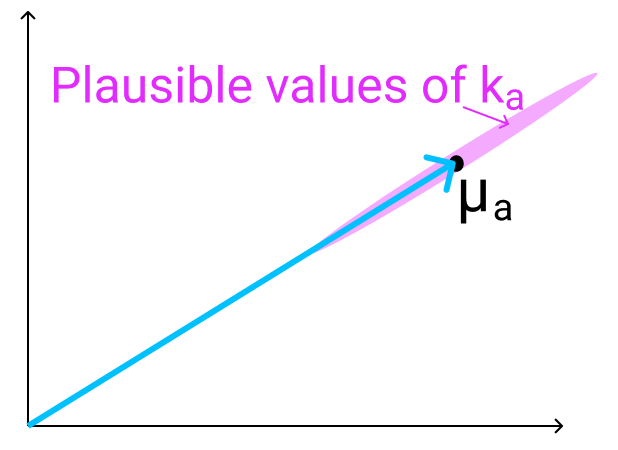
\includegraphics[width=0.35\linewidth]{images/ka_plausible.png}
        \caption{The vector $\mu_a$ (shown here in 2D as an example), with the range of possible values of $k_a$ shown in red. As mentioned previously, $k_a$ points in roughly the same direction as $\mu_a$, but may have larger or smaller magnitude.}
        \label{ka_plausible}
    \end{figure}

    When you sample $\{k_1,\dots,k_n\}$ multiple times, and use the $q$ vector that you defined in part i., what qualitatively do you expect the vector $c$ will look like for different samples?


    \begin{answer}
    % ### START CODE HERE ###
    % ### END CODE HERE ###
    \end{answer}

% \end{subparts}
    \end{enumerate}


% ISS
%\part[3] \textbf{Benefits of multi-headed attention:}
\item \points{3d}  \textbf{Benefits of multi-headed attention:}
Now we'll see some of the power of multi-headed attention.
We'll consider a simple version of multi-headed attention which is identical to single-headed self-attention as we've presented it in this homework, except two query vectors ($q_1$ and $q_2$) are defined, which leads to a pair of vectors ($c_1$ and $c_2$), each the output of single-headed attention given its respective query vector.
The final output of the multi-headed attention is their average, $\frac{1}{2}(c_1+c_2)$.
As in question 3(\ref{q_problem_with_single_head}), consider a set of key vectors $\{k_1,\dots,k_n\}$ that are randomly sampled, $k_i\sim \mathcal{N}(\mu_i, \Sigma_i)$, where the means $\mu_i$ are known to you, but the covariances $\Sigma_i$ are unknown.
Also as before, assume that the means $\mu_i$ are mutually orthogonal; $\mu_i^\top \mu_j = 0$ if $i\not=j$, and unit norm, $\|\mu_i\|=1$.
    % \begin{subparts}
    \begin{enumerate}[label=\roman*.]
    % \subpart[1]
    \item (1 point) Assume that the covariance matrices are $\Sigma_i=\alpha I$, for vanishingly small $\alpha$.
    Design $q_1$ and $q_2$ such that $c$ is approximately equal to $\frac{1}{2}(v_a+v_b)$. 

    \begin{answer}
    % ### START CODE HERE ###
    % ### END CODE HERE ###
    \end{answer}

    % \subpart[2]
    \item (1 points) Assume that the covariance matrices are $\Sigma_a=\alpha I + \frac{1}{2}(\mu_a\mu_a^\top)$ for vanishingly small $\alpha$, and $\Sigma_i=\alpha I$  for all $i \neq a$.
    Take the query vectors $q_1$ and $q_2$ that you designed in part i.
    What, qualitatively, do you expect the output $c$ to look like across different samples of the key vectors? Please briefly explain why. You can ignore cases in which $q_i^\top k_a < 0$.

    \begin{answer}
    % ### START CODE HERE ###
    % ### END CODE HERE ###
    \end{answer}

    \end{enumerate}
    % \end{subparts}

% \part[7]
\item \points{3e} \textbf{Key-Query-Value self-attention in neural networks:}
So far, we've discussed attention as a function on a set of key vectors, a set of value vectors, and a query vector.
In Transformers, we perform \textit{self-attention}, which roughly means that we draw the keys, values, and queries from the same data.
More precisely, let $\{x_1,\dots,x_n\}$ be a sequence of vectors in $\mathbb{R}^d$. 
Think of each $x_i$ as representing word $i$ in a sentence.
One form of self-attention defines keys, queries, and values as follows.
Let $V,K,Q \in \mathbb{R}^{d\times d}$ be parameter matrices. Then
\begin{align}
v_i = Vx_i\ \ i \in \{1,\dots,n\}\\
k_i = Kx_i\ \ i \in \{1,\dots,n\}\\
q_i = Qx_i\ \ i \in \{1,\dots,n\}
%\text{values} &= \{Vx_i, i \in \{1,\dots,n\}\}\\
%\text{keys} &= \{Kx_i, i \in \{1,\dots,n\}\}\\
%\text{queries} &= \{Qx_i, i \in \{1,\dots,n\}\}
\end{align}
Then we get a context vector for each input $i$; we have $c_i = \sum_{j=1}^{n} \alpha_{ij} v_j$, where $\alpha_{ij}$ is defined as $\alpha_{ij} = \frac{\exp(k_j^\top q_i)}{\sum_{\ell=1}^{n}\exp(k_\ell^\top q_i)}$.
Note that this is single-headed self-attention.

In this question, we'll show how key-value-query attention like this allows the network to use different aspects of the input vectors $x_i$ in how it defines keys, queries, and values.
Intuitively, this allows networks to choose different aspects of $x_i$ to be the ``content'' (value vector) versus what it uses to determine ``where to look`` for content (keys and queries.)

    \begin{enumerate}[label=\roman*.]
    % \begin{subparts}
    % \subpart[3]
    \item (1 points) First, consider if we didn't have key-query-value attention. For keys, queries, and values we'll just use $x_i$; that is, $v_i=q_i=k_i=x_i$.
    We'll consider a specific set of $x_i$. In particular, let $u_a,u_b,u_c,u_d$ be mutually orthogonal vectors in $\mathbb{R}^d$, each with equal norm $\|u_a\|=\|u_b\|=\|u_c\|=\|u_d\|=\beta$, where $\beta$ is very large. 
    Now, let our $x_i$ be:
    \begin{align}
    &x_1 = u_d + u_b\\
    &x_2 = u_a \\
    &x_3 = u_c + u_b
    \end{align}
    If we perform self-attention with these vectors, what vector does $c_2$ approximate?
    Would it be possible for $c_2$ to approximate $u_b$ by adding either $u_d$ or $u_c$ to $x_2$? Explain why or why not (either math or English is fine).

    \begin{answer}
    % ### START CODE HERE ###
    % ### END CODE HERE ###
    \end{answer}


    % \subpart[4]
    \item (2 points) Now consider using key-query-value attention as we've defined it originally. Using the same definitions of $x_1$, $x_2$ and $x_3$ as in part i, specify matrices $K,Q,V$ such that $c_2 \approx u_b$, and $c_1\approx u_b - u_c$. There are many solutions to this problem, so it will be easier for you (and the graders), if you first find $V$ such that $v_1 = u_b$ and $v_3 = u_b - u_c$, then work on $Q$ and $K$. Some outer product properties may be helpful (as summarized in this footnote)\footnote{For orthogonal vectors $u,v,w\in\mathbb{R}^d$, the outer product $uv^\top$ is a matrix in $\mathbb{R}^{d\times d}$, and $(uv^\top)v = u(v^\top v)=u\|v\|_2^2$, and $(uv^\top)w = u(v^\top w)=u*0$. (The last equality is because $v$ and $w$ are orthogonal.)}.

    \begin{answer}
    % ### START CODE HERE ###
    % ### END CODE HERE ###
    \end{answer}


    %\ifans{Let $Q=u_bu_a^\top + u_cu_b^\top$, $V=u_bu_b^\top + u_cu_c^\top$, $K=u_bu_b^\top$}
    \end{enumerate}
    % \end{subparts}

%Consider the mutually orthogonal unit vectors $u_1,u_2,u_3$.
%Fix an arbitrary $i \in \{1,\dots,n\}$.


\end{enumerate}
% \end{parts}
